\emph{Random interactions: equilibrium distribution.---}Henceforth we assume $f(x_i)=x_i^{\alpha}$, $g(x_i)=x_i^{\beta}$, $h(x_i)=x_i^{\gamma}$. 
(Any coefficients can be reabsorbed in the statistics of $A$ and by a rescaling of time.)
\begin{figure}[t!]
    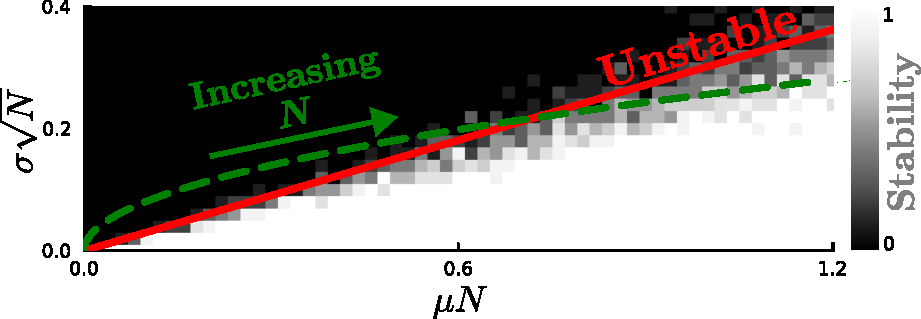
\includegraphics[width=.45\textwidth]{figs/beta1_5-S50-N10-diversity-increase.pdf}
    \caption{For a system in the ``anti-May" phase, an increase in $N$,
    corresponding to moving along $\sqrt{N}$ in the $(\sigma \sqrt{N},\mu N)$ plane (green dashed line), will be stabilizing rather than destabilizing.
    Here we show results from the numerical resolution of the dynamical system~\eqref{dynamics}. Stability is defined as full stable coexistence. The red line is computed obtained using DMFT and the generalized stability condition $N\langle (\sigma/\psi)^2\rangle < 1$.
    Parameters values are $\alpha=1$, $\beta=3/2$,
    $\gamma=1$, $N=50$ and $10$ replicates for the simulations. The green line was plotted for $\mu=0.1$ and $\sigma=0.75$.}
    \label{fig: stability line + sims}
\end{figure}
Following e.g. Ref.~\cite{Roy2019}, we can derive from the evolution equation~\eqref{dynamics} a dynamical mean field theory (DMFT) 
which describes the ensemble of $N\gg 1$ variables
by means of a single, self-consistent representative stochastic trajectory
\begin{equation}
    \dot{x} = x^{\alpha}-A_sx^{\beta+\gamma}-x^{\beta}\big( \mu N \langle x^{\gamma}\rangle + \sigma \sqrt{N} \eta\big) \, ,
\label{eq: dmft}
\end{equation}
where $A_s$ is a random variable with the statistics of $A_{ii}$ and $\eta$ is a Gaussian noise with zero mean and correlation $\langle x^{\gamma}(t)x^{\gamma}(s)\rangle$. 
\begin{figure}[t!]
    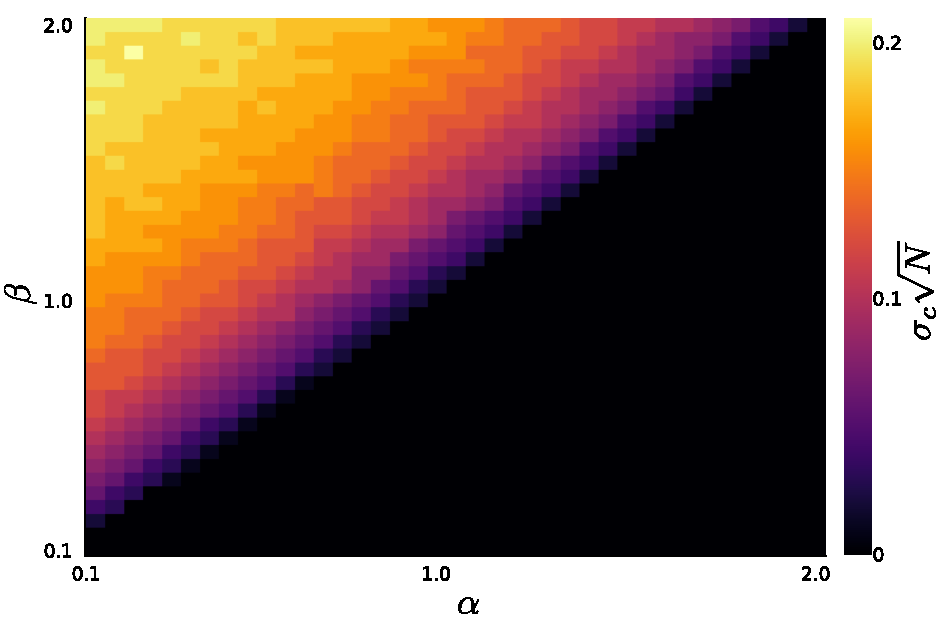
\includegraphics[width=.45\textwidth]{figs/alpha-beta.pdf}
    \caption{The ``May" and ``anti-May" phases derived in the
    case of uniform interactions ($\sigma = 0$) are robust with respect to random interactions ($\sigma > 0$).
    Here we simulated system~\eqref{dynamics} in the power law case for a fixed value of
    $\mu=\mu_s=10^{-2}$, $\gamma=1$, $N=100$ and $100$ replicates,  
    and we evaluated $\sigma_c$, defined here as
    the value above which full stable coexistence is less probable than 50\%,
    at varying $\alpha$ and $\beta$.
    No amount of heterogeneity is allowed in the bottom right triangle because we have $\mu=\mu_s$, while an increasing value of $\sigma_c$
    is found as $\beta$ becomes larger than $\alpha$.
    We stress that the existence of a finite $\sigma_c\sqrt{N}$ above which instability is triggered also in the upper triangle,
    does not imply that increasing $N$ will destabilize the system, because $\mu N$ would also change.
    }
    \label{fig: alpha-beta}
\end{figure}
At equilibrium, we can write
\begin{equation}
    x_*^{\alpha-\beta} - A_s x_*^{\gamma}= \big( \mu N \langle x_*^{\gamma}\rangle + \sigma \sqrt{N\langle x_*^{2\gamma}\rangle}\xi\big) \, ,
\end{equation} 
where $\xi$ is now a standard normal random variable.
The equation above can be solved for $x_*$ for specific values of
$(\alpha-\beta)/\gamma$, or if $A_s=0$.
(In the following we show that neglecting $A_s$ even when it is not zero does not affect noticeably the quality of the approximation.) In this case the stationary solution is given by 
\begin{equation} \label{eq: cavity solution}
    x_* = \left( \mu N \langle x_*^{\gamma}\rangle + \sigma \sqrt{N\langle x_*^{2\gamma}\rangle}\xi\right)^{1/(\alpha-\beta)} \, .
\end{equation}
The equilibrium distribution $P(x_*)$ can then be obtained as the pushforward of the distribution of $\xi$: 
\begin{equation}\label{eq: dist general}
    P(x_*)=\frac{|\alpha-\beta|x_*^{\alpha-\beta-1}}{\sqrt{2\pi\sigma^2 N\langle x_*^{2\gamma}\rangle}}
    \exp{\left\{-\frac{(x_*^{\alpha-\beta}-\mu N\langle x_*^{\gamma}\rangle)^2}{2\sigma^2N\langle x_*^{2\gamma}\rangle}\right\}} \, ,
\end{equation}
where the expectation values must be computed self-consistently. 

Equipped with the equilibrium distribution $P(x^*)$, we can compute, for given $N$ and $\mu$, the maximal heterogeneity $\sigma_c$ compatible with the linear stability condition $N\langle (\sigma/\psi(x^*))^2\rangle < 1$. 

Let us focus on the choice $\alpha=1$, $\beta=3/2$ and $\gamma=1$, with $A_s=0$.  
In this case the first and second moments formally diverge.
This is not truly problematic because we are dealing with large, but \emph{finite} populations.
Following~\cite{Cui2020,Hatton2023} and assuming $\sigma \sqrt{N\langle x_*^2\rangle}\ll \mu N \langle x_* \rangle$, we can expand the solution~\eqref{eq: cavity solution} to first order in $\sigma \sqrt{N\langle x_*^2\rangle}$, and approximate~\eqref{eq: dist general} with a Gaussian distribution with moments $\langle x_*\rangle=(\mu N)^{-2/3}$ and $\langle x_*^2\rangle=(\mu N)^{-4/3}/(1-4(\mu N)^{-2}\sigma^2N)$. 

The result is plotted against simulations in Fig.~\ref{fig: cavity sol.}. We show both the exact solution~\eqref{eq: dist general} (where integration for the moments has been performed up to a maximum value above which no equilibrium value should be found) and the Gaussian approximation. Simulations correspond to $A_s=\mu$, showing that neglecting the $A_s$ term in analytical expressions does not introduce a significant error. 


The properties of large random dynamical systems is often portrayed in the $(\sigma \sqrt{N},\mu N)$ plane \cite{bunin2017ecological}. Everything else being fixed, an increase of the number of degrees of freedom $N$ moves the system along a square-root trajectory in that plane. In the GLV model, the boundary between the stable and unstable parameter regions is the horizontal line $\sigma_c\sqrt{N} = \mu_s$ \cite{bunin2017ecological}, hence stability is never possible at large $N$. 

In Fig.~\ref{fig: stability line + sims} we plot the stability condition $N\langle (\sigma/\psi(x^*))^2\rangle < 1$ for $\alpha = 1$, $\beta = 3/2$ derived from \eqref{eq: dist general} (solid line) together with results from simulations (shading). Here, because the boundary between the stable and unstable phases is a straight line with positive slope, increasing $N$ will eventually bring the system in the stable region. This behavior corresponds to the ``anti-May" phase defined previously. 




Finally, Fig.~\ref{fig: alpha-beta} shows results of simulations for $\sigma_c\sqrt{N}$ in the $(\alpha,\beta)$ plane, at fixed $\mu N$ and $\gamma = 1$. (Numerically, we define $\sigma_c\sqrt{N}$ as the value of $\sigma$ above which full stable coexistence has a probability lower than $50\%$.) In these simulations we use $\mu_s = \mu$, which would never be stable in the GLV model. Fig.~\ref{fig: alpha-beta} illustrates the transition between a ``May" phase for $\alpha \geq \beta$ and an ``anti-May" phase for $\alpha < \beta$, showing that our analytical results are robust to heterogeneous interactions.